
%   Journal Article Template
%%%%%%%%%%%%%%%%%%%%%%%%%%%%%%%%%%%%%%%%%%%%%%%%%%%%%%%%%%%%%%%%%%%%%%%%
\documentclass{siamltex}
\usepackage{graphicx}
\usepackage{amssymb}
\usepackage{bm}
%\usepackage[notref,notcite]{showkeys}
%\usepackage[dvipdfm]{hyperref}
%\usepackage{hyperref}
\usepackage{graphicx}
\usepackage{subfigure}
%\usepackage{epsfig,psfig}
\usepackage{amsfonts,amsmath,latexsym}
\usepackage{amsbsy}


%%%%%%%%%%%%%%%%%%%%%%%%%%%%%%%%%%%%%%%%%%%%%%%%%%%%%%%%%s
%%%%%%%%%%%%%%%%%%%%%%%%%%%%%%%%%%%%%%%%%%%%%%%%%%%%%%%%%%%
%
% PROOF
%
%\newenvironment{rproof}{\addvspace{\medskipamount}\par\noindent{\it Proof:\/}}
%{\unskip\nobreak\hfill$\Box$\par\addvspace{\medskipamount}}
%
% ROMENUM
%
\newcounter{bean}
\newenvironment{romenum}{\begin{list}{{(\roman{bean})}}
{\usecounter{bean}}}{\end{list}}
\newtheorem{remark}[theorem]{Remark}
%
% special SYMBOLS
%
\newcommand{\uu}[1]{\boldsymbol #1}                     % vector fields
\newcommand{\uuu}[1]{\underline{#1}}                 % tensor fields
\newcommand{\jmp}[1]{[\![#1]\!]}                     % jump
\newcommand{\mvl}[1]{\{\!\!\{#1\}\!\!\}}             % mean value
%
% NORMS
%
\newcommand{\N}[1]{\|#1\|}                            % norm
\newcommand{\tn}[1]{|\!|\!|#1|\!|\!|}             % triple norm
%
\newcommand{\mc}[1]{\mathcal{#1}}
\newcommand{\curl}{\rm curl}
\newcommand{\dvr}{\rm div}
%
%%%%%%%%%%%%%%%%%%%%%%%%%%%%%%%%%%%%%%%%%%%%%%%%%%%%%%%%%%%%%%%%%%%%%%%%%%%%%%%%%%%%%%%%%%%%%%%%%
% end: our definitions
%%%%%%%%%%%%%%%%%%%%%%%%%%%%%%%%%%%%%%%%%%%%%%%%%%%%%%%%%%%%%%%%%%%%%%%%%%%%%%%%%%%%%%%%%%%%%%%%%%%






%\newenvironment{Pf}{\noindent {\bf Proof:}} {\hfill $\Box$ \medskip}
%
%%%%%%%%%%%%%%%%%%%%%%%%%%%%%%%%%%%%%%%%%%%%%%%%%%%%%%%%%%%%%%%%%%%%%%%%
%%%%%%%%%%%%%%%%%%%%%%%%%%%%%%%%%%%%%%%%%%%%%%%%%%%%%%%%%%%%%%%%%%%%%%%%


\title{Preconditioners for Mixed Finite Element Discretizations of Incompressible MHD Equations}

\author{
Chen Greif\thanks{Department of Computer Science,
University of British Columbia, Vancouver, BC, V6T 1Z4, Canada,
 greif@cs.ubc.ca.} \and Dan Li \thanks{Microsoft Corporation, email@email.com} \and
 Dominik
Sch\"{o}tzau\thanks{Mathematics Department, University of British
Columbia, Vancouver, BC, V6T 1Z2, Canada,
schoetzau@math.ubc.ca}.
\and Michael Wathen\thanks{Department of Computer Science,
University of British Columbia, Vancouver, BC, V6T 1Z4, Canada,
 mwathen@cs.ubc.ca.}
}





%
%%%%%%%%%%%%%%%%%%%%%%%%%%%%%%%%%%%%%%%%%%%%%%%%%%%%%%%%%%%%%%%%%%%%%%%%
\begin{document}


\maketitle


\begin{abstract}
We consider preconditioning techniques for a discretized incompressible and resistive magnetohydrodynamics problem in mixed form. The governing equations couple the incompressible Navier-Stokes equations with the low-frequency Maxwell equations. We present a few preconditioning ideas for the underlying indefinite linear system, which are based on combining preconditioners for the Maxwell and Navier-Stokes sub-systems. We carry out spectral analysis that demonstrates that the eigenvalues are clustered in some cases. Preliminary numerical results in two dimensions show that our preconditioning techniques are feasible and reasonably scalable.
\end{abstract}

\begin{keywords}
incompressible magnetohydrodynamics, mixed finite element methods, saddle-point linear systems, preconditioners, Krylov subspace methods
\end{keywords}

{\bf REMARKS:}
\begin{itemize}
\item Dan, please add your affiliation details
\item Need to look at the Elman paper and see how the discontinuity of the pressures etc. affects their analysis.
\item In Theorem 4.1 and elsewhere, introduce eigenvectors too in the statement of the theorem(s) and mention geometric multiplicity.
\item Theorem 4.3: refine orthogonality argument in the proof (Helmholtz). First mention Helmholtz and only then the additive relation.
\item Before Theorem 4.4, add remarks that clarify that $n_u-n_b>0$. Clear for 2D, harder for 3D.
\item In numerical experiments refer to our CMAME paper for details, and provide the main details here too. Explain also how initial guess is set.
\item Check literature on preconditioners for div-conforming elements (Zikatanov \& Ayuso)
\item consistency of bib entries
and MHD preconditioners (Elman \& Abner, Zulehner?).
\item Can we show a 3D problem in the numerical experiment section?

\end{itemize}

\section{Introduction}

In our recent work~\cite{Greif10} we introduced and analyzed a mixed finite element method with divergence-free velocities for  the following stationary incompressible and resistive magnetohydrodynamics (MHD) system:
%{\bf [ changed order of equations to $(u,p,b,r)$] }
\begin{subequations}
\label{eq:mhd}
\begin{alignat}2
\label{eq:mhd1} - \nu  \, \Delta\uu{u} + (\uu{u} \cdot \nabla)
\uu{u}+\nabla p - \kappa\,
(\nabla\times\uu{b})\times\uu{b} &= \uu{f} & \qquad &\mbox{in $\Omega$},\\[.1cm]
\label{eq:mhd2}
\nabla\cdot\uu{u} &= 0 & \qquad &\mbox{in $\Omega$},\\[.1cm]
\label{eq:mhd3}
\kappa\nu_m  \, \nabla\times( \nabla\times \uu{b})
+ \nabla r
- \kappa \, \nabla\times(\uu{u}\times \uu{b}) &= \uu{g} & \qquad &\mbox{in $\Omega$},\\[.1cm]
\label{eq:mhd4} \nabla\cdot\uu{b} &= 0 & \qquad &\mbox{in
$\Omega$}.
\end{alignat}
\end{subequations}
Here, $\Omega$ is a bounded simply-connected Lipschitz
polyhedron in~$\mathbb{R}^3$, with a connected
boundary~$\partial\Omega$. The unknowns are the velocity~$\uu{u}$, the hydrodynamic
pressure~$p$, the magnetic field $\uu{b}$, and the Lagrange multiplier $r$
associated with the divergence constraint on the magnetic
field. The functions $\uu{f}$ and $\uu{g}$ represent
external force terms.

The equations \eqref{eq:mhd} are characterized by three
dimensionless parameters: the hydrodynamic Reynolds number ${\rm
Re}=\nu^{-1}$, the magnetic Reynolds number ${\rm
Rm}~=~\nu_m^{-1}$, and the coupling number~$\kappa$. For further
discussion of these parameters and their typical values, we refer
the reader to~\cite{ArmeroSimo96, Gerbeau2006, Roberts67}.

We consider the following homogeneous and inhomogeneous Dirichlet boundary conditions:
\begin{subequations}
\label{eq:bc}
\begin{alignat}2
\label{eq:bc1} \uu{u} &= \uu{0} & \qquad &\mbox{on $\partial\Omega$},\\[.1cm]
\label{eq:bc2}
   \uu{n}\times\uu{b} &= \uu{0} & \qquad &\mbox{on $\partial\Omega$},\\[.1cm]
\label{eq:bc3}      r &=0 &\qquad &\mbox{on $\partial\Omega$},
\end{alignat}
\end{subequations}
with $\uu{n}$ being the unit outward normal on $\partial\Omega$. By taking the
divergence of the magnetostatic equation~(\ref{eq:mhd3}), we
obtain the Poisson problem
\begin{equation}
\label{eq:zero-r} \Delta r =\nabla \cdot \uu{g} \quad \mbox{in
$\Omega$}, \qquad r=0 \quad\mbox{on $\partial\Omega$}.
\end{equation}
Since $\uu{g}$ is divergence-free in physically relevant applications, the multiplier $r$ is typically zero
and its primary purpose is to ensure stability; see also~\cite{Greif10}.

Our goal in this paper is to derive a scalable numerical solution procedure for solving \eqref{eq:mhd}-\eqref{eq:bc}. We first present in Section~\ref{sec:discretization} the finite element discretization and the structure of the matrices that arise throughout the nonlinear iterations. In Section~\ref{sec:preconditioning} we introduce the proposed preconditioners for the indefinite linear systems that arise; our ideas are based on combining preconditioners for the incompressible Navier-Stokes and Maxwell sub-systems appearing  in the MHD system~\eqref{eq:mhd1}--\eqref{eq:mhd4} while taking into account the presence of coupling terms. Spectral analysis is performed in Section~\ref{sec:mhd_eigenvalue}. {\bf [DS: More precise and quote earlier papers]}. In Section~\ref{sec:decoupling} we consider circumstances where the incompressible Navier-Stokes and the Maxwell systems can be decoupled; in such cases the preconditioning approach may be significantly simplified. In Section~\ref{sec:numerical_results_mhd_
solver} we provide preliminary results in two dimensions that show that our numerical  solution techniques are feasible and reasonably scalable. Finally, we offer some concluding remarks in Section~\ref{sec:conclusions}.



\section{Finite element discretization}
\label{sec:discretization}

 In this section, we introduce the mixed finite element discretization proposed in~\cite{Greif10},
 and review the main properties of the resulting numerical scheme.

\subsection{Variational formulation}
\label{sec:variation}

To write~\eqref{eq:mhd} in weak form, we denote by
$(\cdot,\cdot)_\Omega$ the inner product in $L^2(\Omega)$ or
$L^2(\Omega)^3$. Upon introducing the Sobolev spaces
\begin{align*}
\uu{V}&=H^1_0(\Omega)^3=\left\{\,\uu{u}\in H^1(\Omega)^3\,:\,\text{$\uu{u}=\uu{0}$ on $\partial\Omega$}\,\right\},\\[.1cm]
Q&=L^2_0(\Omega)=\{\,p\in L^2(\Omega)\,:\,(p\,,1)_\Omega=0\,\},\\[.1cm]
\uu{C}&=H_0({\rm curl};\Omega) = \left\{\,\uu{b}\in L^2(\Omega)^3\,:\,\nabla\times\uu{b}\in L^2(\Omega)^{3}, \
\text{$\uu{n}\times\uu{b}=\uu{0}$ on $\partial\Omega$}\,\right\},\\[.1cm]
S&=H^1_0(\Omega)=\{\,r\in H^1(\Omega)\,:\,r=0\ \mbox{on
$\partial\Omega$}\,\},
\end{align*}
the variational formulation of the incompressible MHD
system~(\ref{eq:mhd})--(\ref{eq:bc}) amounts to
finding~$(\uu{u},p,\uu{b},r)\in \uu{V} \times Q\times \uu{C} \times
S$ such that
\begin{subequations}
\label{eq:weak}
\begin{eqnarray}
\label{eq:weak1} A(\uu{u},\uu{v}) + O(\uu{u};\uu{u},\uu{v})
+C(\uu{b};\uu{v},\uu{b})
+B(\uu{v}, p) & =& (\uu{f}, \uu{v})_{\Omega},\\[.1cm]
\label{eq:weak2}
B(\uu{u},q)&=&0, \\[.1cm]
\label{eq:weak3}
M(\uu{b},\uu{c})-C(\uu{b};\uu{u},\uu{c})+D(\uu{c},r)&=& (\uu{g},\uu{c})_\Omega, \\[.1cm]
\label{eq:weak4} D(\uu{b},s)&=&0,
\end{eqnarray}
\end{subequations}
for all $(\uu{v},q,\uu{c},s)\in \uu{V} \times Q\times \uu{C}\times
S$. The variational forms are given by
\begin{alignat*}2
&A(\uu{u},\uu{v})=  \int_\Omega \nu \, \nabla\uu{u}:
\nabla\uu{v}\,d\uu{x},&\qquad  & O(\uu{w};\uu{u},\uu{v}) = \int_\Omega
(\uu{w}\cdot\nabla)\uu{u} \cdot\uu{v} \, d\uu{x},
\\[.1cm]
&  B(\uu{u},q) = -\int_\Omega\,(\nabla\cdot\uu{u}) \,q \,d\uu{x},
&\qquad  &
 M(\uu{b},\uu{c})= \int_\Omega\, \kappa\nu_m
(\nabla\times\uu{b})\cdot(\nabla\times\uu{c})\,d\uu{x},\\[0.1cm]
& D(\uu{b},s) = \int_\Omega\, \uu{b} \cdot \nabla s\,
d\uu{x}, & \qquad &
C(\uu{d};\uu{v},\uu{b}) =  \int_\Omega \kappa\, (\uu{v}\times\uu{d})\cdot
(\nabla\times\uu{b})\, d\uu{x}.
\end{alignat*}

The forms $A$, $B$, and $O$ are associated with the variational formulation of the incompressible Navier-Stokes sub-system,
$M$ and $D$ with that of  the Maxwell sub-system in mixed form, and $C$ is the coupling form which combines the two
sub-problems into the full MHD system.
For small data problem~\eqref{eq:weak} is well-posed and has a unique solution; see~\cite{Schoetzau04} for details.


\subsection{Mixed finite elements}

We consider a (family of) regular and quasi-uniform triangulations
${\mathcal T}_h=\{K\}$ of mesh size~$h$ that partition the
domain~$\Omega$ into simplices~$K$. We denote by ${\mathcal F}_h$ the
set of all faces of ${\mathcal T}_h$.
The diameter of a face~$F$ is denoted by~$h_F$.

For $k\geq 1$, we wish to approximate the solution
of~(\ref{eq:mhd})--(\ref{eq:bc}) by finite element
functions~$(\uu{u}_h,p_h,\uu{b}_h,r_h)\in \uu{\cal V}_h\times Q_h\times
\uu{C}_h\times S_h$, where
\begin{equation}
\label{eq:DGspace}
\begin{split}
\uu{V}_h & = \{\, \uu{u}\in H_1( \Omega)\, :\, \uu{u}|_K
\in {\mathcal P}_{k}(K)^3, \, K
\in{\mathcal T}_h \, \},\\[.1cm]
Q_h&=\{\, p\in H_1(\Omega)\,:\, p|_K \in {\mathcal P}_{k-1}(K),
\, K
\in{\mathcal T}_h \,\},\\[.1cm]
\uu{C}_h &=\{\, \uu{b}\in H_0({\rm curl}; \Omega) \,:\, \uu{b}|_K
\in {\mathcal P}_{k-1}(K)^3 \oplus \uu{R}_k(K), \, K
\in{\mathcal T}_h \,\},\\[.1cm]
S_h&=\{\, r\in H_0^1(\Omega) \,:\, r|_K \in {\mathcal P}_{k}(K),
\, K \in {\mathcal T}_h \, \}.
\end{split}
\end{equation}
Here, we denote that we are using Taylor-Hood elements for the velocity and pressure fields proposed in ~\cite{taylor1973numerical}. The
space~$\uu{C}_h$ represents the first family of curl-conforming
N\'{e}d\'{e}lec elements (cf.~\cite[Chapter 5]{Nedelec80}); its
degrees of freedom ensure continuous tangential components of
the discrete magnetic fields across faces. The finite element
spaces~$\uu{V}_h. \, \uu{C}_h, \, Q_h$ and~$S_h$ are conforming subspaces in~$\uu{V}, \, \uu{C}, \,
Q$ and~$S$, respectively.

Now we consider the following finite element method: find
$(\uu{u}_h,p_h,\uu{b}_h,r_h)\in \uu{V}_h\times Q_h\times \uu{C}_h\times S_h$ such that
\begin{subequations}
\label{eq:bn}
\begin{eqnarray}
\label{eq:bn1} A_h(\uu{u}_h,\uu{v}) +
O_h(\uu{u}_h;\uu{u}_h,\uu{v}) +C(\uu{b}_h;\uu{v},\uu{b}_h)
+B(\uu{v}, p_h) & = &
( \uu{f},\uu{v})_\Omega,\\[.1cm]
\label{eq:bn2}
B(\uu{u}_h,q)&=& 0, \\[.1cm]
\label{eq:bn3} M(\uu{b}_h,\uu{c})-C(\uu{b}_h;\uu{u}_h,\uu{c})+
D(\uu{c},r_h)&=& (\uu{g},\uu{c})_\Omega,\\[.1cm]
\label{eq:bn4} D(\uu{b}_h,s)&=&0,
\end{eqnarray}
\end{subequations}
for all $(\uu{v},q,\uu{c},s)\in \uu{V}_h\times Q_h \times \uu{C}_h\times S_h$.

The forms $A, M, B, D$ and $C$ are the same as on the continuous level, whereas $O_h$ are defined in a mesh-dependent manner.
The form $A_h$ associated with the Laplacian is chosen as the
standard interior penalty
form~\cite{Arnold82,ArnoldBrezziCockburnMarini2001}:
\begin{equation*}
\begin{split}
A_h(\uu{u},\uu{v})&=\int_{\Omega}\nu
\nabla_h\uu{u}:\nabla_h\uu{v}\,d\uu{x}- \sum_{F\in{\mathcal
F}_h}\int_{F}\,\mvl{\nu\nabla_h \uu{u}}:
\jmp{\uu{v}}\, ds\\[.1cm]
&-\sum_{F\in {\mathcal F}_h}\int _F\,\mvl{\nu\nabla_h \uu{v}}:
\jmp{\uu{u}}\,ds + \sum_{F\in{\mathcal F}_h} \,\frac{a_0\nu}{h_F}
\int_F\,\jmp{\uu{u}}: \jmp{\uu{v}}\, ds.
\end{split}
\end{equation*}
Here, we use the standard notation $\jmp{\cdot}$ and $\mvl{\cdot}$ for jumps and averages across inter-elemental faces, respectively, with obvious modifications for boundary faces; see~\cite{Greif10}. The operator $\nabla_h$ is the elementwise gradient, and $a_0>0$
is the interior penalty stabilization parameter, which has to be chosen
larger than a threshold value independent
of~$h,\,\nu,\,\kappa$ and~$\nu_m$.

For the convection form, we take
the standard upwind form~\cite{LesaintRaviart74}:
\begin{equation}
\label{eq:upwind-form}
\begin{split}
O_h(\uu{w};\uu{u},\uu{v})=&\int_{\omega}\,(\uu{w}\cdot\nabla)\uu{u}\cdot \uu{v}\,d\uu{x} \\
&+ \int_{\Omega}\, \frac12 (\nabla \cdot \uu{w})\uu{u}\cdot \uu{v} \, dx \\[.1cm]
&-\int_{\partial\Omega}\, \frac12\uu{w}\cdot\uu{n} \, \uu{u} \cdot \uu{v} \, ds.
\end{split}
\end{equation}
Here, $\uu{u}^e$ is the trace of $\uu{u}$ taken from the exterior of
$K$. Notice that due to the presence of the upwind terms the form
$O_h(\uu{w};\uu{u},\uu{v})$ is not linear in the first argument.

This completes the definition of the mixed finite element method introduced in~\cite{Greif10}.

\begin{remark}
\label{remark:MHD-2D}
Let us mention that the finite element method~\eqref{eq:bn} can be readily adapted to two-dimensional versions
of the MHD problem~\eqref{eq:mhd}--\eqref{eq:bc}. In this case, the curl
operator~$\nabla\times$ applied to a vector~$\uu{b}=(b_1, b_2)$ is
defined as $\nabla \times \uu{b} = \frac{\partial b_2}{\partial
x}-\frac{\partial b_1}{\partial y}$, while the curl of a scalar
function~$r$ is determined by $\nabla \times r = (\frac{\partial
r}{\partial y}, -\frac{\partial r}{\partial x}).$ Similarly, the
cross product of two vectors~$\uu{u}=(u_1, u_2)$ and~$\uu{b}=(b_1,
b_2)$ is given by $\uu{u} \times \uu{b} = u_1b_2-u_2b_1$.
\end{remark}


The mixed method~\eqref{eq:bn} has the following main features~\cite{Greif10}, both in two and three dimensions:
\begin{romenum}
\item For small data, there exists a unique discrete solution~$(\uu{u}_h,p_h,\uu{c}_h,r_h)$.
\item  By choosing the divergence-conforming BDM elements as the
approximating space for the velocity, the method~\eqref{eq:bn} gives exactly
divergence-free velocity approximations:
\begin{equation}
\label{eq:div-free}
\nabla\cdot\uu{u}_h \equiv 0\qquad\text{in $\Omega$.}
\end{equation}
Hence, the constraint~\eqref{eq:mhd2} is enforced exactly. As a consequence,
the resulting finite element method is provably energy-stable without the need to skew-symmetrize the convective
discretization.

\item The Lagrange multiplier~$r_h$ is the solution of the discrete Poisson problem
$$
(\nabla r_h, \nabla s)_\Omega= (\uu{g}, \nabla s)_\Omega  \qquad\forall\: s\in S_h.
$$
In particular, it vanishes identically for divergence-free source
terms, thereby mimicking the continuous property
in~(\ref{eq:zero-r}).


\end{romenum}

In~\cite{Greif10}, we also derived nearly optimal a-priori error estimates in the mesh size~$h$
for the errors measured in natural norms for problems with small data. The suboptimality is due to the use of inverse estimates. However, in all
the numerical tests performed in~\cite{Greif10}, we observed optimal convergence rates for
sufficiently smooth solutions, both in two and three dimensions.


\subsection{Matrix form}
\label{sec:bases}

To transform the variational problem~\eqref{eq:bn} into matrix form,
we introce bases for the finite element spaces:
\begin{alignat}2
\label{eq:bases1}
\uu{V}_h & = {\rm span}\langle  \uu{\varphi}_j \rangle _{j=1}^{n_u}, & \qquad &
Q_h  = {\rm span} \langle  \zeta_i \rangle _{i=1}^{m_u},\\[0.1cm]
 \uu{C}_h& ={\rm span}\langle \uu{\psi}_j \rangle _{j=1}^{n_b}, & \qquad & S_h = {\rm span} \langle \phi_i
\rangle_{i=1}^{m_b}.
\end{alignat}
As usual, we then identify finite element functions $(\uu{u}_h, p_h,\uu{b}_h, r_h)\in \uu{V}_h \times Q_h\times \uu{C}_h \times  S_h$ with their coefficient vectors $u = (u_1, \ldots , u_{n_u}) \in \mathbb{R}^{n_u}$, $p = (p_1, \ldots , p_{m_u}) \in \mathbb{R}^{m_u}$,
$b = (b_1, \ldots , b_{n_b}) \in \mathbb{R}^{n_b}$,
and $r = (r_1, \ldots , r_{m_b}) \in \mathbb{R}^{m_b}$, with respect to these bases.
The bilinear forms appearing in~\eqref{eq:bn} now give rise to the following stiffness matrices and load vectors:
\begin{alignat*}2
A_{i,j} &= A_h(\uu{\varphi}_j,\uu{\varphi}_i), &\quad  &1 \leq i,j \leq n_u,\\[0.1cm]
B_{i,j} &= B(\uu{\varphi}_j,\zeta_i), &\quad &1 \leq i \leq m_u, \ 1 \leq j \leq n_u,\\[.1cm]
D_{i,j} &= D(\uu{\psi}_j,\phi_i),  & & 1 \leq i \leq m_b,\ 1 \leq j \leq n_b,\\[.1cm]
M_{i,j}&= M(\uu{\psi}_j,\uu{\psi}_i), &\qquad & 1 \leq i,j \leq n_b,\\[.1cm]
f_i &= (\uu{f},\uu{\varphi}_i)_\Omega, & & 1\leq i\leq n_u,\\[.1cm]
g_i &= (\uu{g},\uu{\psi}_i)_\Omega, & & 1\leq i \leq n_b.
\end{alignat*}
Given two vectors~$w\in\mathbb{R}^{n_u}$ and $d\in\mathbb{R}^{n_b}$ corresponding to finite element functions $\uu{w}\in \uu{V}_h$ and $\uu{d}\in\uu{C}_h$, respectively,
we further define the matrices $O(w)\in\mathbb{R}^{n_u\times n_u}$ and $C(d)\in\mathbb{R}^{n_b\times n_u}$, associated with the convection and coupling forms,
by setting
\begin{alignat*}2
O(w)_{i,j} &=O_h(\uu{w};\uu{\varphi}_j,\uu{\varphi}_i), &\quad  &1 \leq i \leq n_u, \ 1 \leq j \leq n_u,\\[.1cm]
C(d)_{i,j} &= C(\uu{d};\uu{\varphi}_j,\uu{\psi}_i), & & 1\leq i \leq n_b,\ 1 \leq j \leq n_u.
\end{alignat*}

The matrix form of problem~\eqref{eq:bn} then is to find coefficient vectors $u\in\mathbb{R}^{n_u}$, $p\in\mathbb{R}^{m_u}$,  $b\in\mathbb{R}^{n_b}$, and $r\in\mathbb{R}^{m_b}$ such that
\begin{equation}
\label{eq:matrix-system}
\left(
\begin{array}{cccc}
A+O(u) & B^T & C^T(b) & 0\\
B & 0 & 0 & 0\\
-C(b) & 0 & M & D^T \\
0 & 0 & D & 0
\end{array}
\right)
\,
\left(
\begin{array}{c}
u\\
p\\
b\\
r
\end{array}
\right) =
\left(
\begin{array}{c} f\\0\\g\\0
\end{array}
\right).
\end{equation}

\subsection{Nonlinear iterations and linear systems}
\label{subsec:nonlinear_iteration}

We shall find the solution $(\uu{u}_h,
p_h,\uu{b}_h,r_h)$ to the discrete problem~\eqref{eq:bn} through Picard iterations.
If we are given a current iterate $(\uu{u}_h^k,p_h^k,\uu{b}_h^k,r_h^k)$, we shall find updates
$(\delta\uu{u}_h^k,\delta p_h^k,\delta\uu{b}_h^k,\delta r_h^k)$ and define the updated iterate
\begin{alignat*}2
\uu{u}_h^{k+1} &= \uu{u}_h^k+\delta\uu{u}_h^k,& \qquad &
p_h^{k+1} = p_h^k+\delta p_h^{k},\\
\uu{b}_h^{k+1}& =\uu{b}_h^k+\delta\uu{b}_h^k, & &  r_h^{k+1}=r_h^k+\delta r_h^k.
\end{alignat*}
When clear from the context, we will omit the iteration counter~$k$. Analogous notation is used
for the coefficient vectors.

Hence, given the current solution~$(\uu{u}_h,p_h,\uu{b}_h,r_h)$, the Picard iteration (P) consists in finding
updates $(\delta \uu{u}_h,\delta p_h,\delta \uu{b}_h,\delta r_h)\in\uu{V}_h\times Q_h \times\uu{C}_h\times S_h$ such that
\begin{equation}
\label{eq:picard}
\begin{split}
A_h(\delta\uu{u}_h, \uu{v}) +O_h(\uu{u};\delta\uu{u}_h,\uu{v})+ C(\uu{b}_h;\uu{v},\delta \uu{u}_h) + B(\uu{v}, \delta p_h) & = R_u(\uu{u}_h,\uu{b}_h,p_h;\uu{v})\\[.1cm]
B(\delta\uu{u}_h,q)&= R_p(\uu{u}_h;q), \\[.1cm]
M(\delta \uu{b}_h,\uu{c})+
D(\uu{c},\delta r_h)-C(\uu{b}_h;\delta \uu{u}_h,\uu{v})&= R_b(\uu{u}_h,\uu{b}_h,r_h;\uu{c}),\\[.1cm]
D(\delta \uu{b}_h,s)&= R_r(\uu{b}_h;s).
\end{split}
\end{equation}
for all $(\uu{v},q,\uu{c},s)\in\uu{V}_h\times Q_h\times \uu{C}_h\times S_h$, with the residuals given by
\begin{align*}
 R_u(\uu{u}_h,\uu{b}_h,p_h;\uu{v})&=(\uu{f}, \uu{v})_\Omega-A_h(\uu{u}_h,\uu{v})
-  O_h(\uu{u}_h;\uu{u}_h,\uu{v})  - C(\uu{b}_h;\uu{v},\uu{b}_h)-B(\uu{v},p_h),\\[.1cm]
R_p(\uu{u}_h;q)&=-B(\uu{u}_h,q),\\[.1cm]
 R_b(\uu{u}_h,\uu{b}_h,r_h;\uu{c})&=(\uu{g,c})_\Omega -M(\uu{b}_h,\uu{c})
+ C(\uu{b}_h;\uu{u}_h,\uu{c})-D(\uu{c},r_h),\\[.1cm]
R_r(\uu{b}_h;s)&=-D(\uu{b}_h,s).
\end{align*}


Given the coefficient vectors $(u,p,b,r)$ associated with the current iterate, the solution of~\eqref{eq:picard} can now be computed by solving the linear system
\begin{equation}
\label{eq:mhd_saddle}
%\mathcal{K} x \equiv
\left(
\begin{array}{cccc}
A+O(u) & B^T & C^T(b) & 0\\
B & 0 & 0 & 0 \\
-C(b) & 0 & M & D^T\\
0 & 0 & D & 0
\end{array}
\right)
\,
\left(
\begin{array}{c}
\delta u\\
\delta p\\
\delta b\\
\delta r
\end{array}
\right)  =
\begin{pmatrix}
r_u \\
r_p\\
r_b\\
r_r
\end{pmatrix},
\end{equation}
with
\begin{align*}
r_u &= f- Au -O(u) u - C(b)^T b- B^T p,\\[0.1cm]
r_p &=-B u,\\[0.1cm]
r_b &=g-Mu+C(b)b-D^T r,\\[0.1cm]
r_r &=-D b.
\end{align*}


The system~\eqref{eq:mhd_saddle} is in a generalized saddle-point form, and will be the main focus of our analysis. It is nonsymmetric due to the convection term $O$. Note that the part of the matrix involving the skew-symmetric terms  $C(b)$ and $-C(b)^T$ can be easily symmetrized by manipulating signs.

\section{Preconditioning}
\label{sec:preconditioning}
Let us denote the matrix of system \eqref{eq:mhd_saddle} by $\mathcal{K}$. Since the system is typically very large and sparse, we are interested in solving~\eqref{eq:mhd_saddle} iteratively using a preconditioned Krylov subspace solver. As previously discussed, the MHD problem~\eqref{eq:mhd}--\eqref{eq:bc} couples the incompressible Navier-Stokes equations for the fluid variables with a curl-curl Maxwell problem for the magnetic variables. As such, it seems beneficial to devise a preconditioning scheme based on effective preconditioners for the separate sub-problems, and then incorporate the coupling terms.

\subsection{Navier-Stokes preconditioning}

Let us denote the coefficient matrix for the incompressible Navier-Stokes sub-problem by
\begin{equation}
\label{eq:ns_coeff}
\mathcal{K}_{NS}=
\begin{pmatrix}
F & B^T \\
B & 0
\end{pmatrix},
\end{equation}
where $F = A+O$. (In what follows, we shall omit the dependence of $O$ and $C$ on the current iterates $u$ and $b$,
respectively).


An array of excellent preconditioners have been derived for this system; see~\cite{elman-silvester-wathen}. Here we adopt an effective approach based on block upper triangular preconditioners. Suppose $S=B F^{-1} B^T$.
In~\cite{Elman06, Kay02} a block upper triangular that approximates the following matrix is considered:
\begin{equation}
\label{eq:ns_pc_upper}
\mathcal{M}_{\rm NS} =
\begin{pmatrix}
F & B^T \\
0 & -S
\end{pmatrix}.
\end{equation}
In practice the (1,1) block $F$ and the Schur complement matrix $S$ are approximated by matrices that are easier to invert; equivalently, their corresponding approximate inverses are effectively used in the numerical solution process. In Section \ref{XX} we will provide more details on the approach we take to make the Navier-Stokes preconditioner more practical.


For $S$ we will use least-squares commutator preconditioners as proposed in~\cite{ElmanHowle06,Elman06}, which are based on the assumption that
\begin{equation}
\label{eq:ms_ideal}
BF^{-1}B^T \approx  (B Q^{-1} B^T)(BQ^{-1}FQ^{-1}B^T)^{-1}(B Q^{-1} B^T),
\end{equation}
where $Q=(Q_{i,j})_{i,j=1}^{m_u} \in{\mathbb R}^{n_u \times n_u}$ is the velocity mass matrix on $\uu{V}_h$ defined by
\begin{equation}
\label{eq:pressure_mass}
Q_{i,j}=
\int_\Omega\, \uu{\varphi_j} \uu{\varphi_i} \,d\uu{x}, \quad 1\leq i,j \leq n_u.
\end{equation}
{\bf Was talking about pressure mass matrix need to change} \emph{Note, though, that an important difference in our setting compared to that of~\cite{Elman06} is that we have discontinuous pressures and divergence-conforming velocities.
In the lowest order case, the mass matrix $Q$ is diagonal; for higher order elements, it is block diagonal. In the latter case, if necessary $Q$ in \eqref{eq:ms_ideal} can be replaced by $\widehat{Q} = \mathrm{diag}(Q)$ to enhance sparsity; see~\cite[Remark 6.4]{Elman06}. %This gives the following approximation to the Schur complement:
%\begin{equation}
%\label{eq:ms_invert}
%\widehat{S}^{-1} = (B \widehat{Q}^{-1} B^T)^{-1}(B\widehat{Q}^{-1}F\widehat{Q}^{-1}B^T)(B \widehat{Q}^{-1} %B^T)^{-1}.
%\end{equation}
The least-squares commutator preconditioner thus has the form in~\eqref{eq:ns_pc_upper} with~$\widehat{S}$ in~\eqref{eq:ms_invert} as the (2,2) block. Applying this preconditioner involves two Poisson solves (i.e., inversions of $B \widehat{Q}^{-1} B^T$). In our setting these solves involve a nonstandard discontinuous Galerkin type discretization on discontinuous pressures and may entail a larger computational effort compared to the setting described in~\cite{Elman06}. {\bf [DS: Discuss how we solve these? CG: I've added something here. Makes sense?]} That said, given the structure of the discrete operator, a multigrid approach may work effectively here, even though we have not implemented it.
Our numerical results show that this approach performs well for the incompressible Navier-Stokes sub-problem with our particular discretization, though it is not entirely independent of the mesh size.
{\bf [DS: Is it independent for standard FEM? CG: based on our discussion at the time I think not completely but perhaps it is not worth saying too much. I've added the word `entirely' in the last sentence. See if OK.]}}


\subsection{Maxwell preconditioning}

Denote the coefficient matrix for the Maxwell sub-system by
\begin{equation}
\label{eq:maxwell_coeff}
\mathcal{K}_{\rm MX}=
\begin{pmatrix}
M & D^T \\
D & 0
\end{pmatrix}.
\end{equation}

For the Maxwell sub-system, the resulting linear system is associated with the coefficient matrix~\eqref{eq:maxwell_coeff}.
In \cite{Greif07} it was shown that the ideal block diagonal positive definite preconditioner
\begin{equation}
\label{eq:maxwell_pc_ideal}
\mathcal{M}_{\rm idealMX} =
\begin{pmatrix}
M+D^T L^{-1} D & 0 \\
0 & L
\end{pmatrix},
\end{equation}
where $L$ is the scalar Laplacian on~$S_h$ defined as
$L=(L_{i,j})_{i,j=1}^{m_b} \in{\mathbb R}^{m_b \times m_b}$ with
\begin{equation}
\label{eq:scalar_laplace}
L_{i,j}=\int_\Omega\,\nabla\phi_j\cdot\nabla\phi_i\,d\uu{x},
\end{equation}
yields a preconditioned operator with precisely two distinct eigenvalues, $1$ and $-1$, hence a symmetric preconditioned Krylov solver such as MINRES will converge within two iterations in the absence of roundoff errors. However, inverting the (1,1) block of the preconditioner, $M+D^T L^{-1} D$, is typically computationally prohibitive and in practice we use the preconditioner
\begin{equation}
\label{eq:maxwell_pc}
\mathcal{M}_{\rm MX} =
\begin{pmatrix}
\widehat{N} & 0 \\
0 & \widehat{L}
\end{pmatrix},
\end{equation}
where  $\widehat{N}$ is an approximation for $N:=M+X$, where $X=(X_{i,j})_{i,j=1}^{n_b}\in{\mathbb R}^{n_b \times n_b}$ is the
mass matrix on~$\uu{C}_h$, defined as
\begin{equation}
\label{eq:magnetic_mass}
X_{i,j}=\int_\Omega\, \uu{\psi}_j\cdot\uu{\psi}_i\,d\uu{x},
\end{equation}
and $\widehat{L}$ is an approximation for the scalar Laplacian $L$. Multigrid approaches have been proven to be effective here as approximations; see \cite{XX,XX,XX}.

The preconditioner $\mathcal{M}_{\rm MX}$ is considerably easier to deal with compared to  \eqref{eq:maxwell_pc_ideal}, and it still has rather attractive spectral properties; in particular, the preconditioned operator $\mathcal{M}_{MX}^{-1} \mathcal{K}_{\rm MX}$ has the two eigenvalues $1$ and $-1$ with algebraic multiplicity $m_b$  each, and the rest of the eigenvalues are bounded by a constant independent of the mesh size; cf.~\cite{Greif07}. We thus will use $\mathcal{M}_{\rm MX}$ as a preconditioner for the Maxwell sub-problem.  A scalable implementation strategy of these approximations has been proposed in~\cite{LiGreifSchoetzauNLA}; it is based on {[\bf MORE: HiptmairXu...]}

\subsection{MHD preconditioning}

Let us now denote by ${\mathcal K}_{\rm MH}$ the full MHD matrix in~\eqref{eq:mhd_saddle}.
Equipped with the above preconditioners ${\mathcal M}_{\rm NS}$
in~\eqref{eq:ns_pc_upper}
and ${\mathcal M}_{\rm MX}$ in~\eqref{eq:maxwell_pc} for the incompressible Navier-Stokes and the Maxwell problems, respectively,
we incorporate the coupling terms and propose the following preconditioner for
iteratively solving the system with~${\mathcal K}_{\rm MH}$.  From here on, we shall neglect the approximations $\widehat{F}$, $\widehat{N}$, and $\widehat{L}$, and in our notation we will use $F, N$ and $S$, with the understanding that in practice, approximations are to be used. We get
\begin{equation}
\label{eq:mhd_pc_ls}
\mathcal{M}_{\rm MH} =
\left(
\begin{array}{cccc}
F & B^T & C^T & 0\\
0 & -S & 0 & 0 \\
-C & 0 & N & 0\\
0 & 0 & 0 & L
\end{array}
\right),
\end{equation}
with the matrices defined in the preceding sections.


To further facilitate the solution procedure, we will consider
solving linear systems associated with $\mathcal{M}_{\rm MH}$ using the following inner preconditioner:
\begin{equation}
\label{eq:mhd_pc_inner}
\mathcal{M}_{\rm IMH} =
\left(
\begin{array}{cccc}
F & B^T & 0 & 0\\
0 & -\widehat{S} & 0 & 0 \\
0 & 0 & N & 0\\
0 & 0 & 0 & L
\end{array}
\right).
\end{equation}
We provide some  eigenvalue analysis for this preconditioning approach in Section~\ref{sec:mhd_eigenvalue}.

%\subsection{Applying the least-squares (LS) preconditioner to the entire MHD system}
%
%We end this section with comments on the idea of treating the entire MHD system as a saddle-point system. Indeed, after reordering the equations the system~\eqref{eq:mhd_saddle} can be written as
%\begin{equation}
%\label{eq:mhd_saddle_ns}
%\left(
%\begin{array}{cccc}
%F & C^T & B^T & 0\\
%-C & M & 0 & D^T \\
%B & 0 & 0 & 0\\
%0 & D & 0 & 0
%\end{array}
%\right)
%\,
%\left(
%\begin{array}{c}
%\delta u\\
%\delta b\\
%\delta p\\
%\delta r
%\end{array}
%\right) =
%\left(
%\begin{array}{c} r_u\\r_b\\r_p\\r_r
%\end{array}
%\right).
%\end{equation}
%
%Let us rewrite the coefficient matrix in~\eqref{eq:mhd_saddle_ns} as a $2\times 2$ block matrix as the following system
%\begin{equation}
%\label{eq:mhd_saddle_ns2}
%\begin{pmatrix}
%\mathcal{F} & \mathcal{B}^T \\
%\mathcal{B} & 0
%\end{pmatrix},
%\end{equation}
%where
%\begin{equation*}
%\label{eq:mhd_F}
%\mathcal{F} =
%\begin{pmatrix}
%F & C^T \\
%-C & M
%\end{pmatrix} ,
%\qquad
%\mathcal{B} =
%\begin{pmatrix}
%B & 0 \\
%0 & D
%\end{pmatrix}.
%\end{equation*}
%
%Note that the matrix~\eqref{eq:mhd_saddle_ns2} has the same form as that in~\eqref{eq:ns_coeff}. Our finite element formulation is inf-sup stable;
%see~\cite[Section~3.3]{Greif10}. The operator~$\mathcal{F}$ has a component~$F$, which is a convection-diffusion type operator. Assuming that $\mathcal{F}$ preserves some properties of a convection-diffusion operator, we consider applying the least-squares commutator preconditioner directly to the entire discretized MHD system. The preconditioner is
%\begin{equation}
%\label{eq:mhd_pc_all}
%\mathcal{M}_{\rm LS} =
%\begin{pmatrix}
%\mathcal{F} & \mathcal{B} \\
%0 & -\widehat{\mathcal{S}}
%\end{pmatrix}.
%\end{equation}
%Here $\mathcal{S}$ is defined as
%\begin{equation*}
%\widehat{\mathcal{S}} = (\mathcal{B} \widehat{\mathcal{Q}}^{-1} \mathcal{B}^T)^{-1}(\mathcal{B}\widehat{\mathcal{Q}}^{-1}\mathcal{F}\widehat{\mathcal{Q}}^{-1}\mathcal{B}^T)(\mathcal{B} \widehat{\mathcal{Q}}^{-1} \mathcal{B}^T)^{-1},
%\end{equation*}
%where
%$$\widehat{\mathcal{Q}} = \mathrm{diag}
%\begin{pmatrix}
%Q & 0 \\
%0 & X
%\end{pmatrix}.
%$$
%
%As we briefly show in the numerical experiments section, it seems that this approach does not yield a scalable solver (see Tables \ref{tab:smooth_iterations_pa} and \ref{tab:singular_iterations_pa} in Section \ref{sec:numerical_results_mhd_solver}), and we will not pursue it in terms of spectral analysis. {\bf [Does it work with $\mathcal Q$? Instead of taking the diagonal of $X$, it might
%be better to do mass lumping.]}


\section{Spectral analysis}
\label{sec:mhd_eigenvalue}

In this section, we provide an eigenvalue analysis for the preconditioner~$\mathcal{M}_{\rm MH}$ in~\eqref{eq:mhd_pc_ls}.

\subsection{Discrete Helmholtz decomposition}

{\bf [DS: I've decided to move this here]}
Our analysis relies on the discrete Helmholtz decomposition for the magnetic spaces $\uu{C}_h\times S_h$; cf.~\cite{asdf}.  To state this decomposition in terms of discrete operators, we follow~\cite[Section~2]{Greif07}, and note that $\mathbb{R}^{n_b}$ can now be written as the direct sum
\begin{equation}
\label{eq:helmholtz}
\mathbb{R}^{n_b}={\rm null}(M)\oplus {\rm null}(D).
\end{equation}
Vectors $b\in{\rm null}(M)$ are referred to as discrete gradients, and vectors in ${\rm null}(D)$
as discretely divergence-free magnetic fields. Indeed, for $b\in{\rm null}(M)$, there
is a unique $q\in\mathbb{R}^{m_b}$ such that $b=G r$ where $G\in\mathbb{R}^{n_b\times m_b}$ is the discrete gradient matrix given by
\begin{equation}
\label{eq:gradient}
\nabla \phi_j=\sum_{i=1}^{n_b} G_{i,j} \uu{\psi}_i, \qquad j=1,\ldots,m_b.
\end{equation}
The decomposition~\eqref{eq:helmholtz} is $X$-orthogonal. That is, if $b=b_M+b_D$, then
\begin{equation}
\label{eq:orth}
\langle Xb, b_M\rangle=\langle X b_M, b_M \rangle,\qquad \langle Xb, b_D\rangle= \langle X b_D,b_D\rangle.
\end{equation}



\subsection{An ideal preconditioner}

We start our analysis with an ideal version of~\eqref{eq:mhd_pc_ls}, $\mathcal{M}_{\rm idealMH}$, which corresponds
to combining ${\mathcal M}_{\rm NS}$ in \eqref{eq:ns_pc_upper} with $F$ replacing $\widehat{F}$, together with ${\mathcal M}_{\rm idealMX}$ in~\eqref{eq:maxwell_pc_ideal}, along with the coupling terms: % to precondition the Maxwell sub-system:
\begin{equation}
\label{eq:mhd_pc_ideal}
\mathcal{M}_{\rm idealMH} =
\left(
\begin{array}{cccc}
F & B^T & C^T & 0\\
0 & -\widehat{S} & 0 & 0 \\
-C & 0 & M + D^T L^{-1} D & 0\\
0 & 0 & 0 & L
\end{array}
\right).
\end{equation}


\begin{theorem}
\label{thm:mhd_outer_ideal}
The matrix $\mathcal{M}_{\rm idealMH}^{-1} \mathcal{K}_{\rm MH} $ has an eigenvalue $\lambda = 1$ with algebraic multiplicity of at least $n_u + n_b$ and an eigenvalue $\lambda = -1$ with  algebraic multiplicity of at least $m_b$. The eigenvector corresponding to $\lambda=1$ is: $(u, -\widehat{S}^{-1} B u, b, L^{-1} D b)$ with $u$ anything.
\end{theorem}

\begin{proof}
The corresponding eigenvalue problem is
 \begin{equation*}
 \hspace{-3mm}   % Chen: a small manipulation to avoid black thick vertical line; remove later
\left(
\begin{array}{cccc}
F & B^T & C^T & 0\\
B & 0 & 0& 0\\
-C & 0& M & D^T\\
0 & 0 & D & 0
\end{array}
\right)
\left(
\begin{array}{c}
u\\
p\\
b\\
r
\end{array}
\right)
=
\lambda \left(
\begin{array}{cccc}
F & B^T &C^T & 0\\
0 & -\widehat{S} & 0 & 0\\
-C &0 & M+D^T L^{-1} D & 0\\
0 & 0 &  0 & L
\end{array}
\right)
\left(
\begin{array}{c}
u\\
p\\
b\\
r
\end{array}
\right).
\end{equation*}
The four block rows can be written as
\begin{eqnarray}
\label{eq:outer_row1_ideal} (1-\lambda) (Fu + B^T p+ C^T b) &=& 0,\\
\label{eq:outer_row2_ideal} B u &=& -\lambda \widehat{S}\, p,\\
\label{eq:outer_row3_ideal} (\lambda -1) C u + (1 - \lambda) M b - \lambda D^T L^{-1} D b + D^T r &=& 0,\\
\label{eq:outer_row4_ideal} D b &=& \lambda L r.
\end{eqnarray}

If $\lambda = 1$, \eqref{eq:outer_row1_ideal} is satisfied automatically and \eqref{eq:outer_row2_ideal} yields
$p = -\widehat{S}^{-1} B u.$
Equation~\eqref{eq:outer_row4_ideal} leads to $r = L^{-1} D b.$
If this holds, \eqref{eq:outer_row3_ideal} is readily satisfied.
Therefore, $(u, -\widehat{S}^{-1} B u, b, L^{-1} D b)$ is an eigenvector corresponding to $\lambda=1$. There exist $n_u$ linearly independent such $u$'s and $n_b$ linearly independent such $b$'s. There are at least $n_u+n_b$ linearly independent nonzero vectors satisfying the eigenvalue problem when $\lambda = 1$. It follows that $\lambda = 1$ is an eigenvalue with algebraic multiplicity of at least $n_u + n_b$.

If $\lambda = -1$, \eqref{eq:outer_row4_ideal} leads to $r = -L^{-1} D b.$
Substituting it into~\eqref{eq:outer_row3_ideal}, we obtain $Cu = Mb.$ If $b=Gs$ is a discrete gradient, with the gradient matrix~$G$ defined in~\eqref{eq:gradient}, then $Mb = 0$ and $C^T b = 0$. If we take $u=0$, then $Cu = 0$ and the requirement $Cu = Mb$ is satisfied.
If $u=0$ and $b=Gs$ is a discrete gradient, equation~\eqref{eq:outer_row1_ideal} becomes $B^Tp = 0$. Since $B$ has full row rank, this implies $p=0$.

Therefore, if $b=Gs$ is a discrete gradient, then $(0, 0, Gs, -L^{-1}D Gs)$ is an eigenvector corresponding to $\lambda = -1$. According to the discrete Helmholtz decomposition~\eqref{eq:helmholtz}, there are $m_b$ discrete gradients. Therefore $\lambda = -1$ is an eigenvalue with algebraic multiplicity at least  $m_b$.
\end{proof}

\begin{remark}
In our experiments, we have observed the eigenvalue $\lambda = 1$ has algebraic multiplicity of exactly $n_u+n_b$ and the eigenvalue $\lambda = -1$ has algebraic multiplicity of exactly $m_b$. Proving this may be difficult, though, due to complicated generalized eigenvalue problems that arise in the calculation.
\end{remark}

Theorem~\ref{thm:mhd_outer_ideal} shows that $\mathcal{M}_{\rm idealMH}^{-1} \mathcal{K}_{\rm MH}$ has tightly clustered eigenvalues $\lambda=\pm 1$.  Since we have provided explicit expressions for the eigenvectors associated with $\lambda= \pm 1$, we know that the geometric multiplicities of these two eigenvalues are equal to their algebraic multiplicity.
We thus expect a good convergence behavior for  $\mathcal{M}_{\rm idealMH}^{-1} \mathcal{K}_{\rm MH}$.

\subsection{The preconditioner ${\mathcal M}_{\rm X}$}

Next, we replace in the Maxwell sub-system the ideal preconditioner ${\mathcal M}_{\rm idealMX}$ in~\eqref{eq:maxwell_pc_ideal} Theorem~\ref{thm:mhd_outer_ideal} by its practical version~${\mathcal M}_{\rm MX}$ in~\eqref{eq:maxwell_pc}.

\begin{theorem}
\label{thm:mhd_outer}
The matrix $\mathcal{M}_{\rm MH}^{-1} \mathcal{K}_{\rm MH}$ has an eigenvalue $\lambda = 1$ with algebraic multiplicity of at least $n_u+m_b$ and an eigenvalue $\lambda = -1$ with  algebraic multiplicity of at least $m_b$. {\bf [State eigenvectors]}
\end{theorem}

\begin{proof}
The corresponding eigenvalue problem is
 \begin{equation*}
 %\hspace{-3mm}
\left(
\begin{array}{cccc}
F & B^T & C^T & 0\\
B & 0 & 0& 0\\
-C & 0& M & D^T\\
0 & 0 & D & 0
\end{array}
\right)
\left(
\begin{array}{c}
u\\
p\\
b\\
r
\end{array}
\right)
=
\lambda \left(
\begin{array}{cccc}
F & B^T &C^T & 0\\
0 & -\widehat{S} & 0 & 0\\
-C &0 & N & 0\\
0 & 0 &  0 & L
\end{array}
\right)
\left(
\begin{array}{c}
u\\
p\\
b\\
r
\end{array}
\right).
\end{equation*}
Noting that $N=M+X$, the four block rows can be written as
\begin{eqnarray}
\label{eq:outer_row1} (1-\lambda) (Fu + B^T p+ C^T b) &=& 0,\\
\label{eq:outer_row2} B u &=& -\lambda \widehat{S}\, p,\\
\label{eq:outer_row3} (\lambda -1) C u + (1 - \lambda) M b - \lambda X b + D^T r &=& 0,\\
\label{eq:outer_row4} D b &=& \lambda L r.
\end{eqnarray}

If $\lambda = 1$, \eqref{eq:outer_row1} is satisfied automatically and \eqref{eq:outer_row2} yields
$p = -\widehat{S}^{-1} B u.$
Let us examine in what circumstances \eqref{eq:outer_row3} is satisfied.
The first two terms in that equation, namely $(\lambda -1) C u + (1 - \lambda) M b$, vanish for $\lambda=1$.  By~\eqref{eq:outer_row4} we have $r = L^{-1} D b$, and hence we seek vectors that satisfy (for $\lambda=1$)
\begin{equation}
\label{eq:DLXcondition}
  X b = D^T L^{-1} D b .
  \end{equation}
To that end, we write $b=b_M+b_D$ according to~\eqref{eq:helmholtz}, with $b_M \in {\rm null}(M)$ and $b_D \in {\rm null}(D)$. Then from the orthogonality~\eqref{eq:orth} and~\cite[Corollary~3.2]{Greif07}, we have that
$$
\langle Xb ,b_M\rangle=\langle X b_M, b_M \rangle = \langle D^T L^{-1} D b_M, b_M \rangle.
$$
{\bf [Here, we actually need~\eqref{eq:orth} since we seek $b$'s for which \eqref{eq:DLXcondition} holds.]}
Hence, equation~\eqref{eq:DLXcondition} is automatically satisfied for any vector $b=b_M \in {\rm null}(M)$. Since there are $m_b$ null vectors, the algebraic multiplicity of the eigenvalue $\lambda=1$ is at least $1$. Then
$(u, -\widehat{S}^{-1} B u, b_M, L^{-1} D b_M)$ is an eigenvector corresponding to $\lambda=1$. There exist $n_u$ linearly independent such $u$'s and $m_b$ linearly independent such $b_M$'s. There are at least $n_u+m_b$ linearly independent nonzero vectors satisfying the eigenvalue problem when $\lambda = 1$. Therefore $\lambda = 1$ is an eigenvalue with algebraic multiplicity of at least $m_b + n_u$.

If $\lambda = -1$, \eqref{eq:outer_row4} again leads to $r = -L^{-1} D b, $ and
substituting it into~\eqref{eq:outer_row3}, we obtain $$Cu = Mb.$$ If $b=Gs$ is a discrete gradient, $Mb = 0$ and $C^T b = 0$. If we take $u=0$, then $Cu = 0$ and the requirement $Cu = Mb$ is satisfied.


If $u=0$ and $b$ is a discrete gradient, \eqref{eq:outer_row1} becomes $$B^Tp = 0.$$ Since $B$ has full row rank, this implies $p=0$.
Therefore, if $b$ is a discrete gradient, $(0, 0, b, -L^{-1}D b)$ is an eigenvector corresponding to $\lambda = -1$. In view of~\eqref{eq:helmholtz}, there are $m_b$ discrete gradients. Therefore $\lambda = -1$ is an eigenvalue with algebraic multiplicity at least  $m_b$.
\end{proof}


\subsection{The inner preconditioner $\mathcal{M}_{\rm  IMH}$}

Next, we perform some eigenvalue analysis for the inner GMRES iterations based
on $\mathcal{M}_{\rm IMH}$ in~\eqref{eq:mhd_pc_inner}.

\begin{theorem}
\label{thm:mhd_inner}
The matrix $\mathcal{M}_{\rm IMH}^{-1} \mathcal{M}_{\rm MH} $ has an eigenvalue $\lambda = 1$ with algebraic multiplicity of at least $m_u + n_u + 3m_b - n_b$.
 {\bf [State eigenvectors. Discuss positivity of $n_u-n_b$?]}
\end{theorem}

\begin{proof}
The corresponding eigenvalue problem is
\begin{equation*}
\left(
\begin{array}{cccc}
F & B^T & C^T & 0\\
0 & -\widehat{S} & 0& 0\\
-C & 0& N & 0\\
0 & 0 & 0 & L
\end{array}
\right)
\left(
\begin{array}{c}
u\\
p\\
b\\
r
\end{array}
\right)
=
\lambda \left(
\begin{array}{cccc}
F & B^T &0 & 0\\
0 & -\widehat{S} & 0 & 0\\
0 &0 & N & 0\\
0 & 0 &  0 & L
\end{array}
\right)
\left(
\begin{array}{c}
u\\
p\\
b\\
r
\end{array}
\right).
\end{equation*}
The four block rows can be written as
\begin{eqnarray}
\label{eq:inner_row1} (1-\lambda)Fu +(1-\lambda)B^T p+ C^T b &=& 0,\\
\label{eq:inner_row2} (1-\lambda) \widehat{S} \,p &=& 0,\\
\label{eq:inner_row3} -C u + (1 - \lambda) (M+X) b  &=& 0,\\
\label{eq:inner_row4} (1-\lambda)L r &=& 0.
\end{eqnarray}
If $\lambda = 1$, \eqref{eq:inner_row2} and \eqref{eq:inner_row4} are satisfied automatically.
Equation~\eqref{eq:inner_row1} becomes
$$C^T b = 0.$$
If $b=Gs$ is a discrete gradient, this is satisfied and~\eqref{eq:inner_row3} becomes
$$Cu=0, $$ thus we need to require that $u$ be in the null space of $C$.
Therefore, $(u, p, b, r)$ is an eigenvector associated with eigenvalue $\lambda = 1$, if $u$ is in the null space of $C$ and $b$ is a discrete gradient.  The matrix $C$ is $n_b \times n_u$, so we have
\begin{eqnarray}
\label{eq:rank_nullity_Ct} \mathrm{rank}(C^T) + \mathrm{nullity}(C^T) &=& n_b,\\
\label{eq:rank_nullity_C} \mathrm{rank}(C) + \mathrm{nullity}(C) &=& n_u.
\end{eqnarray}
Here nullity refers to the dimension of the null space.
There are exactly $m_b$ distinct discrete gradients due to~\eqref{eq:helmholtz}. The nullity of $C^T$ is at least $m_b$. According to~\eqref{eq:rank_nullity_Ct}, the rank of $C^T$ is at most $n_b-m_b$. Matrix $C$ has the same rank as $C^T$. According to~\eqref{eq:rank_nullity_C}, the nullity of $C$ is at least $n_u-n_b+m_b$. We have $m_u$ linearly independent $p$ in $Q_h$ and $m_b$ linearly independent $r$ in $S_h$. So, there are at least $m_u + n_u + 3m_b - n_b$ linearly independent eigenvectors. Therefore, the eigenvalue $\lambda = 1$ has algebraic multiplicity of at least $m_u + n_u + 3m_b - n_b$.
\end{proof}



\section{Decoupling}
\label{sec:decoupling}

The MHD problem combines an incompressible Navier-Stokes sub-system and a  Maxwell sub-system with coupling terms.  The skew-symmetric form in which the coupling matrix $C$ appears and the nonsymmetry of the convection term make the linear system solve throughout the nonlinear iterations rather challenging.
If the coupling is not very strong, we can treat it explicitly, and call this situation {\em magnetic decoupling}.
Then the Navier-Stokes and Maxwell sub-systems are decoupled, and we apply the specialized preconditioners discussed in Section~\ref{sec:preconditioning} separately.
We will also consider the case where both the coupling and convection terms are treated explicitly, referred to as {\em complete
decoupling}. In terms of preconditioning, this is the simplest case: it amounts to precondition a Stokes problem
and a Maxwell curl-curl problem in mixed form.


\subsection{Magnetic decoupling (MD)}

In the case of weak coupling, we take the coupling terms explicitly and obtain the following iteration.
Given $(\uu{u}_h,p_h,\uu{b}_h,r_h)$, the updates  solve the decoupled system: find  $(\delta \uu{u}_h,\delta p_h,\delta \uu{b}_h,\delta r_h)\in\uu{V}_h\times Q_h\times \uu{C}_h\times S_h$ such that
\begin{equation}
\label{eq:picard_explicit_C}
\begin{split}
A_h(\delta\uu{u}_h, \uu{v}) +O_h(\uu{u};\delta\uu{u}_h,\uu{v})+ B(\uu{v}, \delta p_h) & = R_u(\uu{u}_h,\uu{b}_h,p_h;\uu{v})\\[.1cm]
B(\delta\uu{u}_h,q)&= R_p(\uu{u}_h;q), \\[.1cm]
M(\delta \uu{b}_h,\uu{c})+
D(\uu{c},\delta r_h)&= R_b(\uu{u}_h,\uu{b}_h,r_h;\uu{c}),\\[.1cm]
D(\delta \uu{b}_h,s)&=R_r(\uu{b}_h;s),
\end{split}
\end{equation}
for all $(\uu{v},q,\uu{c},s)\in\uu{V}_h\times Q_h\times\uu{C}_h\times S_h$, with the residual forms
defined in Section~\ref{subsec:nonlinear_iteration}.

The corresponding coefficient matrix is now of the form
\begin{equation}
\label{eq:matrix_MD}
\mathcal{K}_{\rm MD} =
\left(
\begin{array}{cccc}
F & B^T & 0 & 0\\
B & 0 & 0 & 0 \\
0 & 0 & M & D^T\\
0 & 0 & D & 0
\end{array}
\right).
\end{equation}
It is still nonsymmetric, but the two sub-systems are decoupled. If we refer to \eqref{eq:matrix_MD} as a $2 \times 2$ block matrix, then the (1,1) block corresponds to the incompressible Navier-Stokes sub-system and the (2,2) block corresponds to the Maxwell sub-system. We can apply GMRES preconditioned with \eqref{eq:ns_pc_upper} to the (1,1) block and apply MINRES preconditioned with \eqref{eq:maxwell_pc} to the (2, 2) block. That is, as follows from our discussion in Section \ref{sec:preconditioning}, we can apply GMRES with the following preconditioner:
\begin{equation}
\label{eq:mhd_pc_explicit}
\mathcal{M}_{\rm MD} =
\left(
\begin{array}{cccc}
F & B^T & 0 & 0\\
0 & -\widehat{S} & 0 & 0 \\
0 & 0 & N & 0\\
0 & 0 & 0 & L
\end{array}
\right).
\end{equation}

\subsection{Complete decoupling (CD)}

The simplest strategy is to take all the non-linear terms explicitly. Hence, given $(\uu{u}_h,p_h,\uu{b}_h,r_h)$, the updates  solve the system: find  $(\delta \uu{u}_h,\delta p_h,\delta \uu{b}_h,\delta r_h)\in\uu{V}_h\times Q_h\times \uu{C}_h\times S_h$ such that
\begin{equation}
\label{eq:picard_explicit_OC}
\begin{split}
A_h(\delta\uu{u}_h, \uu{v}) + B(\uu{v}, \delta p_h) & = R_u(\uu{u}_h,\uu{b}_h.p_h;\uu{v})\\[.1cm]
B(\delta\uu{u}_h,q)&= R_p(\uu{u}_h;q), \\[.1cm]
M(\delta \uu{b}_h,\uu{c})+
D(\uu{c},\delta r_h)&= R_b(\uu{u}_h,\uu{b}_h,r_h;\uu{c}),\\[.1cm]
D(\delta \uu{b}_h,s)&=R_r(\uu{b}_h;s),
\end{split}
\end{equation}
for all $(\uu{v},q, \uu{c},s)\in\uu{V}_h\times Q_h\times \uu{C}_h\times S_h$.

The coefficient matrix associated with this nonlinear iteration is of the form
\begin{equation}
\label{eq:matrix_CD}
\mathcal{K}_{\rm CD} =
\left(
\begin{array}{cccc}
A & B^T & 0 & 0\\
B & 0 & 0 & 0 \\
0 & 0 & M & D^T\\
0 & 0 & D & 0
\end{array}
\right),
\end{equation}
corresponding to a decoupled Stokes problem and a curl-curl problem in mixed form.

We can use a symmetric solve and apply MINRES to both of the sub-systems. For the Stokes sub-system, we opt to use a standard block diagonal and symmetric positive definite preconditioner of the form
\begin{equation*}
\label{eq:mhd_pc_explicit2_1}
\begin{pmatrix}
A & 0 \\
0 & \widehat{S}
\end{pmatrix}.
\end{equation*}
A natural choice for $\widehat{S}$ is $\widehat{S} = \frac{1}{\nu}Q$, where $Q$ is the pressure mass matrix in~\eqref{eq:pressure_mass}. This preconditioner allows one to obtain mesh-independent convergence rates;
see~\cite{Elman96,Klawonn99}. For the Maxwell sub-system, we use the preconditioner~\eqref{eq:maxwell_pc}.

Altogether, we apply MINRES with the preconditioner
\begin{equation}
\label{eq:mhd_pc_explicit2}
\mathcal{M}_{\rm CD} =
\left(
\begin{array}{cccc}
A & 0 & 0 & 0\\
0 & \widehat{S} & 0 & 0 \\
0 & 0 & N & 0\\
0 & 0 & 0 & L
\end{array}
\right).
\end{equation}




\section{Numerical results}
\label{sec:numerical_results_mhd_solver}

In this section we present a series of
numerical experiments.
We use inner-outer Krylov iterations to solve for the updates in each Picard-type iteration step.
In all experiments, which are carried out using
{\textsc{Matlab}}, the relative
residual of the outer iterations is set to $1e-6$ and the relative residual of the inner iterations
is set to $1e-8$. The tolerance for the Picard-type iteration is chosen as $1e-5$ {\bf [in which norms?]}.
Throughout this section, the lowest order BDM and N\'{e}d\'{e}lec
elements are employed and the interior penalty stabilization
parameter is $a_0 = 10$.

We test our method on problems with mixed Dirichlet and Neumann
boundary conditions in the hydrodynamic variables, even though the
analysis has been carried out solely for the Dirichlet case.
Throughout this section, $\Gamma_N$ denotes the Neumann boundary,
and $\Gamma_D$ the Dirichlet boundary. On Neumann boundaries, we
specify the value of~$(p\underline{\uu{I}}-\nu \nabla\uu{u})
\uu{n}$, where~$\underline{\uu{I}}$ is the identity matrix.

{\bf [Say something about tildes?]}


For the outer iterations, we show the iteration counts in the last Picard step. For the inner iterations, we show the iteration counts for the last inner iteration. In the numerical experiments,  we denote by (P),  (MD), and  (CD) the standard Picard linearization in~\eqref{eq:picard}, and the magnetic decoupling linearization in~\eqref{eq:picard_explicit_C} and complete decoupling linearization~\eqref{eq:picard_explicit_OC}, respectively.

\subsection{Example 1: A two-dimensional problem with a smooth solution}


In this example we consider the following two-dimensional problem. We set $\Omega =
(-1, 1)^2$ with $\Gamma_N = \{(1, y) : y\in (-1, 1)\}$, $\Gamma_D =
\partial \Omega \backslash \Gamma_N$, $\nu = \kappa =1$, $\nu_m
=\rm{1e4}$, and choose the source terms~$\uu{f}$, $\uu{g}$ and the
boundary conditions so that the analytical solution is of the form
\begin{align*}
\uu{u}(x,y)& =(y^2, x^2),&
p(x,y)& =x,\\[0.1cm]
\uu{b}(x,y)& =(1-y^2, 1-x^2),& r(x,y)& =(1-x^2)(1-y^2).
\end{align*}

{\bf STILL MISSING: INITIAL GUESS. DESCRIPTION OF MESHES.}

Table~\ref{tab:smooth_picard} shows the number of non-linear iterations required for the different linearization schemes {\bf [What is the tolerance?]}
The symbol "nc" indicates the linearization does not converge. We run the experiments with different values of~$\nu$. Note that~$\nu$ only shows up in front of the diffusion operator~$A$ and reducing it, both the convection and the coupling get relatively stronger.

Table~\ref{tab:smooth_picard} shows that when the convection and coupling get stronger, the completely decoupled linearization (CD) in~\eqref{eq:picard_explicit_OC} does not converge, while the other two schemes do converge. In this example,
scheme (MD) in~\eqref{eq:picard_explicit_C} behaves like the standard Picard linearization (P) as the numbers of steps required to converge by these two schemes are the same.

\begin{table}[!ht]
\begin{center}
\begin{tabular}{ccccccccccccccc}
\hline
&\multicolumn{3}{l}{$\nu = 1$} & \multicolumn{3}{l}{$\nu = 0.1$} & \multicolumn{3}{l}{$\nu = 0.01$} \\
  DOFs& (P) & (MD) & (CD) & (P) & (MD) & (CD) & (P) & (MD) & (CD)\\
\hline
169 & 5 & 5 & 5 & 8 & 8 & nc & 13 & 13 & nc \\
721 & 5 & 5 & 5 & 9 & 9 & nc & 15 & 15 & nc \\
2,977 & 5 & 5 & 5 & 9 & 9 & nc & 15 & 15 & nc \\
12,097 & 5 & 5 & 5 & 8 & 8 & nc & 14 & 14 & nc \\
\hline
\end{tabular}
\caption{Example 1. Nonlinear iteration counts for various values of $\nu$. We denote by (P) the standard Picard linearization in~\eqref{eq:picard}, and by (MD) and (CD) the linearizations in~\eqref{eq:picard_explicit_C} and~\eqref{eq:picard_explicit_OC}, respectively.}
\label{tab:smooth_picard}
\end{center}
\end{table}

If we treat the coupling terms explicitly using the linearization (MD), the linear system fully decouples into an
incompressible Navier-Stokes problem and a Maxwell system. These can now be solved for separately. Table~\ref{tab:smooth_iterations_pe} shows the iteration counts for the two sub-problems based on the preconditioner ${\mathcal M}_{\rm MD}$ in~\eqref{eq:mhd_pc_explicit}. That is, the incompressible Navier-Stokes sub-system is iteratively solved with GMRES using the least-squares commutator preconditioner~$\mathcal{M}_{\rm NS}$ in~\eqref{eq:ns_pc_upper},~\eqref{eq:ms_invert}.
We denote by $its_1$ the number of GMRES iterations.
The Maxwell system is solved with MINRES with the block diagonal preconditioner in \eqref{eq:maxwell_pc}. We dnote by $its_2$ the number of such MINRES iterations.
When the mesh is refined, more GMRES iterations are required, while the number of MINRES iterations remains the same. This shows that our Maxwell preconditioner is independent of the mesh size, as shown in~\cite{Greif07} for the Maxwell problem in isolation, while the Navier-Stokes preconditioner is not (yet it is not very sensitive to a change of the mesh size).
When the convection and coupling get stronger, typically more iterations are required.
The fast convergence of the Maxwell problem can be attributed to the fact that the eigenvalues appear in two extremely tight clusters.

\begin{table}[!ht]
\begin{center}
\begin{tabular}{cccccccccccccccccccccccccccccccccccccccccc}
\hline
& \multicolumn{2}{l}{$\nu=1$} & \multicolumn{2}{l}{$\nu=0.1$} & \multicolumn{2}{l}{$\nu=0.01$} \\
DOFs & $its_1$ & $its_2$ & $its_1$ & $its_2$ & $its_1$ & $its_2$\\
\hline
169 & 28 & 2 & 27 & 2 & 24 & 2\\
721 & 51 & 2 & 48 & 2 & 57 & 2 \\
2,977 & 58 & 2 & 58 & 2 & 85 & 2\\
12,097 & 66 & 2 & 65 & 2 & 99 & 2\\
\hline
\end{tabular}
\caption{Example 1. Magnetic decoupling (MD): Iteration counts for various values of $\nu$.}
\label{tab:smooth_iterations_pe}
\end{center}
\end{table}

When both the coupling and convection terms are treated explicitly using linearization scheme (CD), we run MINRES iterations for both the Stokes and Maxwell sub-problems based on
the preconditioner $\mathcal{M}_{CD}$ in~\eqref{eq:mhd_pc_explicit2}.
In Table~\ref{tab:smooth_iterations_ps}, we show the corresponding MINRES iteration counts.
When the mesh is refined, we observe that the number of iteration counts for the Stokes problem slightly increases, while that for the Maxwell system remains the same.
{\bf [DS: Shouldn't the Stokes preconditioner be independent of the mesh size? Comment.]}
Notice that the completely decoupled scheme only converges for $\nu=1$, while
it breaks down for smaller values of~$\nu$.

\begin{table}[!ht]
\begin{center}
\begin{tabular}{cccccccccccccccccccccccccccccccccccccccccc}
\hline
& \multicolumn{2}{l}{$\nu=1$} & \multicolumn{2}{l}{$\nu=0.1$} & \multicolumn{2}{l}{$\nu=0.01$} \\
DOFs & $its_1$ & $its_2$ & $its_1$ & $its_2$ & $its_1$ & $its_2$\\
\hline
169 & 38 & 2 & nc & nc & nc & nc\\
721 & 42 & 2 & nc & nc & nc & nc \\
2,977 & 44 & 2 & nc & nc & nc & nc\\
12,097 & 54 & 2 & nc & nc & nc & nc\\
\hline
\end{tabular}
\caption{Example 1. Complete decoupling (CD): Iteration counts for various values of $\nu$.}
\label{tab:smooth_iterations_ps}
\end{center}
\end{table}

Table \ref{tab:smooth_iterations_pc} shows the inner and outer GMRES iteration counts, using the outer preconditioner $\mathcal{M}_{\rm MH}$ in~\eqref{eq:mhd_pc_ls} and the inner preconditioner $\mathcal{M}_{\rm IMH}$ in~\eqref{eq:mhd_pc_inner}. Here, $its$ denotes the number of outer GMRES iterations, and $its_i$ denotes the number of inner GMRES iterations. When the mesh is refined, the outer GMRES solve requires more iterations and the iteration counts are comparable to the iteration counts for the Navier-Stokes sub-system in Table~\ref{tab:smooth_iterations_pe}. The preconditioner $\mathcal{M}_{\rm MH}$ is not independent of the mesh size, but it is not very sensitive to the change. When $\nu$ decreases, more outer iterations are required. The inner iterations show mesh-size independent behavior and they are not sensitive to a change of $\nu$, either.

\begin{table}[!ht]
\begin{center}
\begin{tabular}{cccccccccccccccccccccccccccccccccccccccccc}
\hline
& \multicolumn{2}{l}{$\nu=1$} & \multicolumn{2}{l}{$\nu=0.1$} & \multicolumn{2}{l}{$\nu=0.01$} \\
DOFs & $its$ & $its_i$ & $its$ & $its_i$ & $its$ & $its_i$\\
\hline
169 & 29 & 3 & 28 & 4 & 26 & 5\\
721 & 54 & 3 & 52 & 3 & 61 & 5 \\
2,977 & 62 & 3 & 63 & 3 & 94 & 4\\
12,097 & 75 & 3 & 70 & 3 & 110 & 4\\
\hline
\end{tabular}
\caption{Example 1. Inner and outer iteration counts for various values of $\nu$, using $\mathcal{M}_{\rm MH}$.}
\label{tab:smooth_iterations_pc}
\end{center}
\end{table}

The real eigenvalues of the preconditioned linear system~${\mathcal{M}}_{\rm idealMH}^{-1} \mathcal{K}$ are shown in Figure~\ref{fig:pc_inner_eigs_smooth}.
%Figure~\ref{fig:pc_inner_eigs_smooth} shows the real eigenvalues of the preconditioned linear system~$\widehat{\mathcal{P}}_C^{-1} \mathcal{K}$.
%We assume an eigenvalue is real, if the magnitude of its imaginary part is less then $1e-10$.
In this experiment, we take $\nu=1$ and use a mesh with 721 degrees of freedom, which corresponds to $n_b=176$, $m_b=49$, $n_u = 368$ and $m_u =128$.  According to Theorem~\ref{thm:mhd_outer}, we expect to see $\lambda=1$ with algebraic multiplicity of at least $n+n_u = 544$ and $\lambda=-1$ with algebraic multiplicity of at least $m = 49$. In our experiment, we obtain
$\lambda = 1$ with algebraic multiplicity of exactly 544, and $\lambda = -1$ with algebraic multiplicity of exactly 49. For the inner preconditioner, we expect to see $\lambda = 1$ with algebraic multiplicity of at least $m_u + n_u + 3m_b - n_b = 467$ of the preconditioned linear system $\mathcal{M}_{\rm IMH}^{-1} \mathcal{M}_{\rm MH}$. Numerically, we obtain 469 real eigenvalues and they are all 1.


\begin{figure}[ht]
\begin{center}
\begin{tabular}{cc}\\
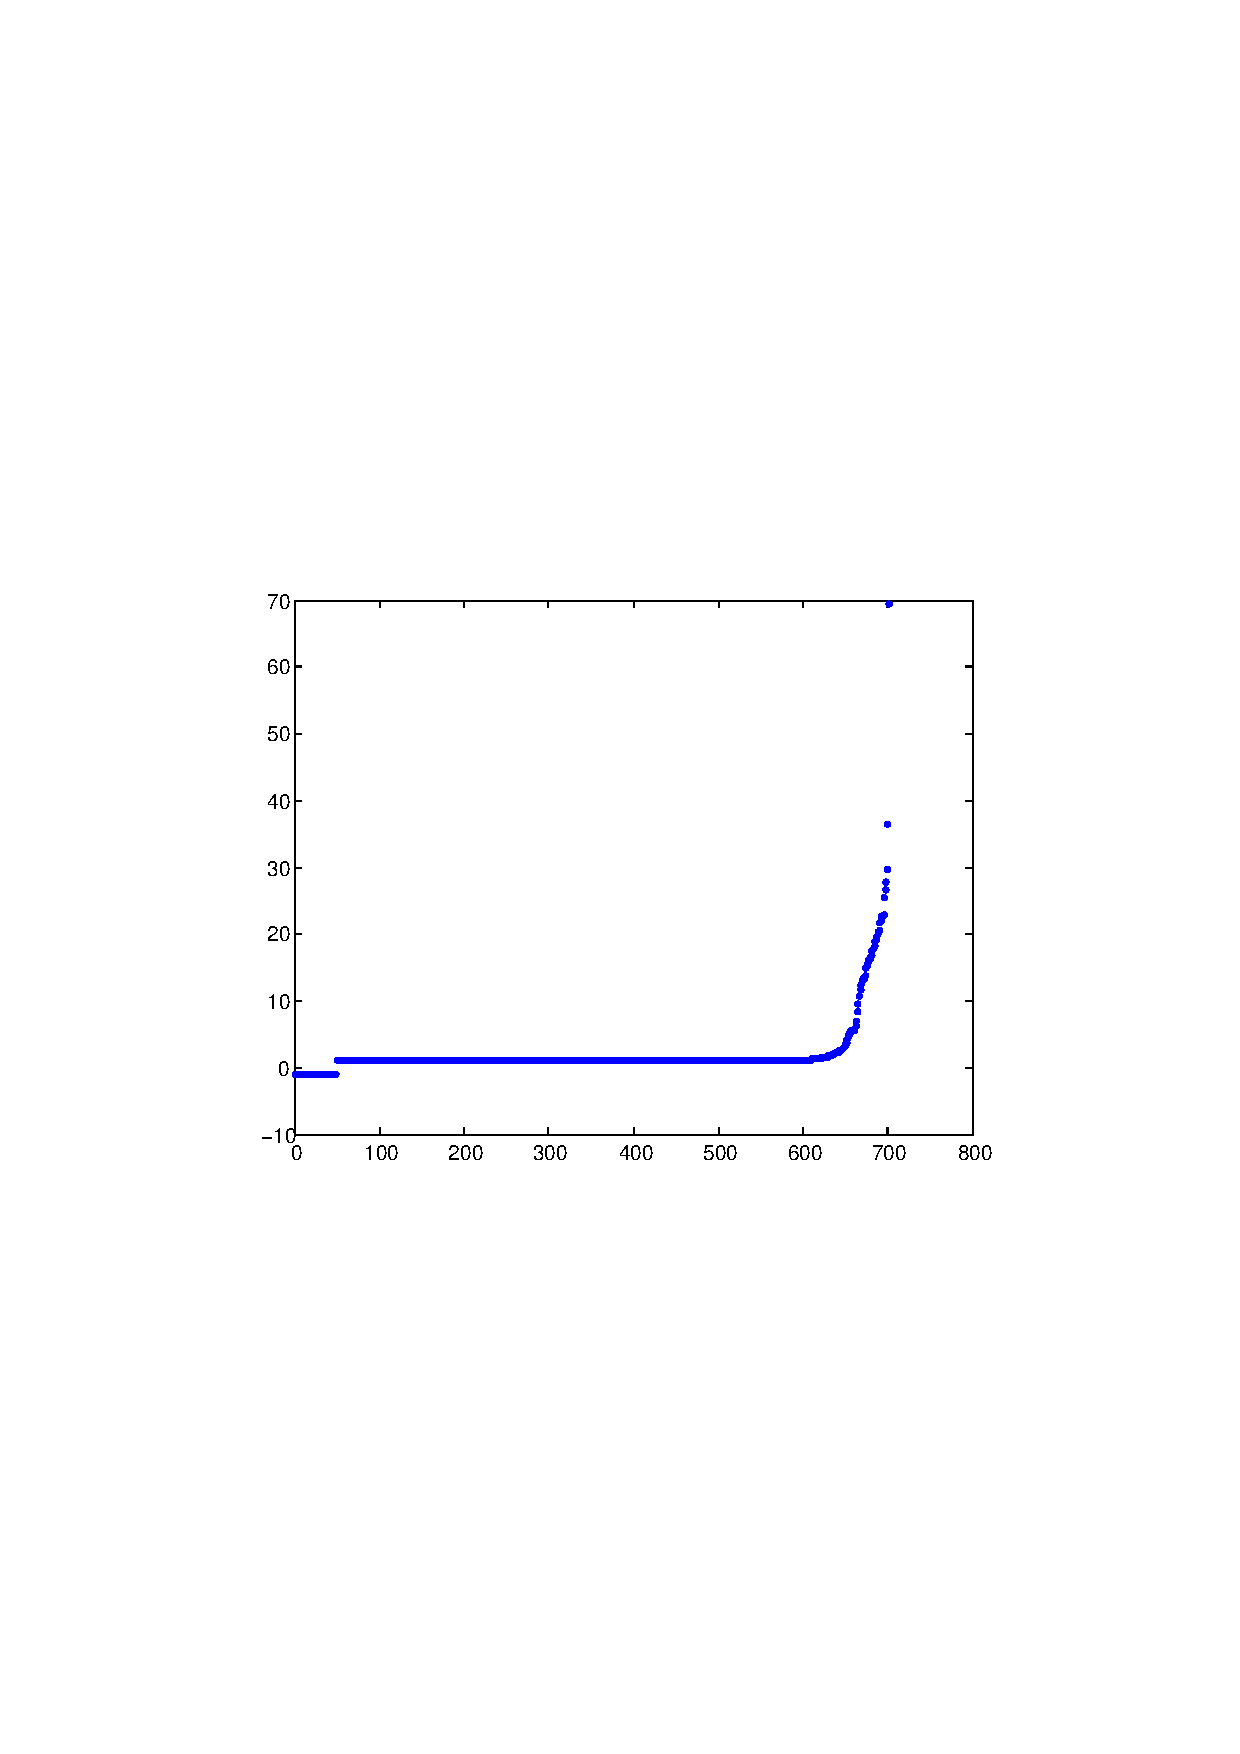
\includegraphics[width=0.9\textwidth]{figs/smooth_outer_eigs_N8.pdf}
\end{tabular}
\end{center}
\caption {Example 1. Plot of the eigenvalues of the preconditioned matrix $\mathcal{M}_{\rm idealMH}^{-1} \mathcal{K}$, $\mathrm{DOFs} = 721$.}
\label{fig:pc_inner_eigs_smooth}
\end{figure}


Table~\ref{tab:smooth_iterations_pa} shows iteration counts for GMRES preconditioned with $\mathcal{M}_{\rm LS}$. The number of iteration counts grows up very quickly, as we refine the mesh. This preconditioning approach is more sensitive to a change of the mesh size, compared with the previous approaches. Evidently, this approach is less effective in the current setting.


\begin{table}[!ht]
\begin{center}
\begin{tabular}{ccccccccccccccc}
\hline
DOFs& $\nu = 1$ & $\nu = 0.1$ & $\nu = 0.01$ \\
\hline
169 & 37 & 35 & 33 \\
721 & 98 & 97 & 106\\
2,977 & nc & 283 & 310 \\
12,097 & nc & nc & nc\\
\hline
\end{tabular}
\caption{Example 1. Iteration counts for various values of $\nu$, using $\mathcal{M}_{\rm LS}$.}
\label{tab:smooth_iterations_pa}
\end{center}
\end{table}



\subsection{Example 2: two-dimensional problem with a singular solution}


In order to verify the capability of the proposed method to capture
singularities in two dimensions, we consider a problem in the
L-shaped domain $\Omega=(-1,1)^2\setminus ([0,1)\times (-1,0])$ with
$\Gamma_N = \{(1, y) : y\in (0, 1)\}$, $\Gamma_D = \partial \Omega
\backslash \Gamma_N$, and set $\nu = \kappa = 1$, $\nu_m =\rm{1e4}$.
We choose the forcing terms and the boundary conditions such that
the analytic solution is given by the strongest corner singularities
for the underlying elliptic operators. In polar coordinates
$(\rho,\theta)$, the hydrodynamic solution components~$\uu{u}$ and~$p$
are then given by
\begin{equation*}
\begin{split}
\uu{u}(\rho,\theta) &=
\begin{bmatrix}
\rho^\lambda((1+\lambda)\sin(\theta)\xi(\theta)+\cos(\theta)\xi^{\prime}(\theta))\\[.1cm]
\rho^\lambda(-(1+\lambda)\cos(\theta)\xi(\theta)+\sin(\theta)\xi^{\prime}(\theta))
\end{bmatrix},\\[0.1cm]
p(\rho,\theta) &=
-\rho^{\lambda-1}((1+\lambda)^2\xi^{\prime}(\theta)+\xi^{\prime\prime
\prime}(\theta)) /(1-\lambda),
\end{split}
\end{equation*}
where
\begin{alignat*}1
\xi(\theta) =& \sin((1+\lambda)\theta)\cos(\lambda \omega)/(1+\lambda) -
\cos((1+\lambda)\theta) \\[0.1cm]
 &-\sin((1-\lambda)\theta)\cos(\lambda
\omega)/(1-\lambda)+\cos((1-\lambda)\theta),
\end{alignat*}
$\omega=\frac{3}{2}\pi$ and~$\lambda \approx 0.54448373678246$. The
magnetic pair $(\uu{b},r)$ is given by
$$\uu{b}(\rho,\theta)= \nabla(\rho^{2/3} \sin{(2/3\theta)}), \qquad r(\rho,\theta)\equiv 0.$$


For this example, we have that
$(\uu{u},p)~\in~H^{1+\lambda}(\Omega)^2~\times~ H^{\lambda}(\Omega)$
and $\uu{b} \in H^{2/3}(\Omega)^2$. Note that straightforwardly
applied nodal elements cannot correctly resolve the magnetic field.
In \cite{XXX} we
investigated the asymptotic rates of convergence of the errors in the
approximations of the hydrodynamic and magnetic variables and
observed that the discrete solution converges to the exact one as the
mesh size $h$ approaches zero, in accordance with our analysis. The results showed full agreement with the
optimal rates for $\| \uu{u}-\uu{u}_h \|_{1,h}$ and~$\|
\uu{b}-\uu{b}_h \|_{H(\curl;\Omega)}$. For the pressure, we also observed
that the rate for $\|p-p_h\|_{L^2(\Omega)}$ is approaching the
optimal rate, albeit more slowly. Additionally, we observed
the~$L^2$-norm of $r$ is zero because $\uu{g}$ is divergence-free.
{\bf [Discuss meshes. initial guess]}
Table~\ref{tab:singular_picard} shows the number of iterations required for different Picard-type linearization schemes. Again, we observe that scheme (CD), which is the Picard-type linearization in \eqref{eq:picard_explicit_OC}, converges more slowly than the other two linearization schemes. If the coupling and convection get stronger, this linearization does not converge.
Scheme (MD) given in~\eqref{eq:picard_explicit_C} shows a similar behavior to the standard Picard linearization. However, because the convection term is treated explicitly in this scheme, it will fail to converge if convection is strong. Indeed, for this example, taking $\nu = 0.01$, $\nu_m = 1\mathrm{e}4$ and $\kappa = 1\mathrm{e}6$, scheme (CD) fails to converge, while (P) and (MD) still converge.

\begin{table}[!ht]
\begin{center}
\begin{tabular}{ccccccccccccccc}
\hline
&\multicolumn{3}{l}{$\nu = 1$} & \multicolumn{3}{l}{$\nu = 0.1$} & \multicolumn{3}{l}{$\nu = 0.01$} \\
 DOFs& (P) & (MD) & (CD) & (P) & (MD) & (CD) & (P) & (MD) & (CD) \\
\hline
117 & 4 & 4 & 7 & 6 & 6 & nc & 8 & 8 & nc \\
521 & 5 & 5 & 9 & 7 & 7 & nc & 10 & 10 & nc \\
2,193 & 4 & 4 & 9 & 8 & 8 & nc & 10 & 10 & nc \\
8,893 & 4 & 4 & 9 & 7 & 7 & nc & 11 & 11 & nc \\
\hline
\end{tabular}
\caption{Example 2. Picard-type iteration counts for various values of $\nu$. We denote by (P) the standard Picard linearization in~\eqref{eq:picard}, by (MD) and (CD) the Picard-type linearizations in~\eqref{eq:picard_explicit_C} and~\eqref{eq:picard_explicit_OC}, respectively.}
\label{tab:singular_picard}
\end{center}
\end{table}

Table \ref{tab:singular_iterations_pe} shows the iteration counts for the two sub-problems, when the coupling terms are treated explicitly. Here, we also find that the least-squares commutator preconditioner is not completely independent of the mesh size, but it is not very sensitive to a change of the mesh size. For the Maxwell sub-problem, our scheme is not sensitive to a change of the mesh size.

\begin{table}[!ht]
\begin{center}
\begin{tabular}{cccccccccccccccccccccccccccccccccccccccccc}
\hline
& \multicolumn{2}{l}{$\nu=1$} & \multicolumn{2}{l}{$\nu=0.1$} & \multicolumn{2}{l}{$\nu=0.01$} \\
DOFs & $its_1$ & $its_2$ & $its_1$ & $its_2$ & $its_1$ & $its_2$\\
\hline
117 & 22 & 1 & 20 & 1 & 18 & 1\\
521 & 46 & 1 & 50 & 1 & 40 & 1 \\
2,193 & 56 & 1 & 84 & 1 & 83 & 1\\
8,893 & 63 & 1 & 88 & 1 & 99 & 1\\
\hline
\end{tabular}
\caption{Example 2. Iteration counts for various values of $\nu$. The coupling terms are treated explicitly.}
\label{tab:singular_iterations_pe}
\end{center}
\end{table}

Table \ref{tab:singular_iterations_pc} shows the inner and outer GMRES iteration counts, using the outer preconditioner $\mathcal{M}_{\rm MH}$ in~\eqref{eq:mhd_pc_ls} and the inner preconditioner $\mathcal{M}_{\rm IMH}$ in~\eqref{eq:mhd_pc_inner}. The outer iterations demonstrate a similar behavior to the iterations of the Navier-Stokes sub-system in Table~\ref{tab:singular_iterations_pe}. The inner iterations are not sensitive to a change of the mesh size and $\nu$.

\begin{table}[!ht]
\begin{center}
\begin{tabular}{cccccccccccccccccccccccccccccccccccccccccc}
\hline
& \multicolumn{2}{l}{$\nu=1$} & \multicolumn{2}{l}{$\nu=0.1$} & \multicolumn{2}{l}{$\nu=0.01$} \\
DOFs & $its$ & $its_i$ & $its$ & $its_i$ & $its$ & $its_i$\\
\hline
117 & 22 & 3 & 20 & 3 & 18 & 3\\
521 & 46 & 3 & 50 & 3 & 41 & 3 \\
2,193 & 56 & 3 & 84 & 3 & 89 & 3\\
8,893 & 68 & 3 & 106 & 3 & 138 & 3\\
\hline
\end{tabular}
\caption{Example 2. Inner and outer iteration counts for various values of $\nu$, using $\mathcal{M}_{\rm MH}$.}
\label{tab:singular_iterations_pc}
\end{center}
\end{table}

Table~\ref{tab:singular_iterations_pa} shows iteration counts for GMRES preconditioned with $\mathcal{M}_{\rm LS}$. Here, similarly to the previous example, we also find that the iteration does not scale very well when we refine the mesh.

\begin{table}[!ht]
\begin{center}
\begin{tabular}{ccccccccccccccc}
\hline
DOFs& $\nu = 1$ & $\nu = 0.1$ & $\nu = 0.01$ \\
\hline
117 & 27 & 25 & 23\\
521 & 79 & 83 & 73\\
2,193 & 217 & 245 & 244\\
8,893 & nc & nc & nc\\
\hline
\end{tabular}
\caption{Example 2. Iteration counts for various values of $\nu$, using $\mathcal{M}_{\rm LS}$.}
\label{tab:singular_iterations_pa}
\end{center}
\end{table}

\section{Concluding remarks}
\label{sec:conclusions}
We have considered preconditioners for the discrete three different approaches for combining the preconditioners
for the sub-systems. We choose the preconditioner based on how strong the convection and coupling are. If they are not very strong, we take an approach whereby preconditioners for the sub-systems are combined together directly without coupling. If the coupling terms are small, we can treat them explicitly. As shown in Tables~\ref{tab:smooth_picard} and \ref{tab:singular_picard}, the linearization scheme (MD) requires the same iterations as the standard Picard linearization (P).  If both of the coupling and convection terms are negligible,  we can treat both of them explicitly as in scheme (CD). When the mesh is refined, schemes (MD) and (CD) are not completely mesh-independent, but they are not very sensitive to a change of the mesh size. However, if the coupling and convection are strong, these schemes will converge more slowly compared with the standard Picard scheme, or may not converge. We propose to combine the preconditioners for the sub-systems with the coupling terms as in $\mathcal{M}_{\rm MH}$. As shown in Tables~\ref{tab:smooth_iterations_pc} and \ref{tab:singular_iterations_pc}, this approach performs qualitatively similarly to the least-squares commutator preconditioner for the Navier-Stoke sub-problem shown in Tables~\ref{tab:smooth_iterations_pe} and \ref{tab:singular_iterations_pe}. A different approach, where the least-squares commutator is applied to the entire discretized MHD system, does not work as well as the other approaches, as shown in Tables~\ref{tab:smooth_iterations_pa} and \ref{tab:singular_iterations_pa}.

The difficulty with the preconditioner $\mathcal{M}_{\rm MH}$ is that solving systems associated with it is non-trivial because the coupling terms destroy the block diagonal structure. To deal with this, we have shown that adding a layer of  inner iterations with inner block diagonal preconditioners proves to be relativey effective.

The approach we have taken seems promising in terms of scalability. Future work will test this for significantly larger problems. {\bf [new, but needs more:]} This also involves designing and numerically testing effective approximations $\widehat{F}$, $\widehat{N}$, and $\widehat{L}$,
which we neglected in this work.

\bibliographystyle{plain}
\bibliography{refs_combine,ref_michael}

\end{document}






